% 引入导言区
\documentclass[10pt]{book}
\usepackage{ctex}
\usepackage{amsmath, amsthm, amssymb, amsfonts}
\usepackage{thmtools}
\usepackage[dvipsnames]{xcolor}
\usepackage{tcolorbox}
\tcbuselibrary{skins,breakable,theorems}
\usepackage{hyperref}
\usepackage{fontspec}
\usepackage{tikz}
\usepackage{fancyhdr}
\pagestyle{fancy}
\usetikzlibrary{arrows.meta, positioning}

% -------------------------------
% 全局正文字体（英文 + 中文） + 伪粗体
% -------------------------------
\setmainfont{Times New Roman}
\setCJKmainfont{SimSun}[AutoFakeBold={3}]
\setCJKfamilyfont{theoremCJK}{FangSong}[AutoFakeBold={2.5}]
\setCJKfamilyfont{proofCJK}{KaiTi}[AutoFakeBold={2.5}]
\newcommand{\theoremFont}{\CJKfamily{theoremCJK}}

% 证明字体
\newcommand{\proofFont}{\CJKfamily{proofCJK}}

% -------------------------------
% 鲜明蓝色系配色方案
% -------------------------------
\definecolor{LogicBlue}{RGB}{0, 102, 204}
\definecolor{LogicLightBlue}{RGB}{102, 204, 255}
\definecolor{LogicDarkBlue}{RGB}{0, 51, 153}
\definecolor{LogicAccentBlue}{RGB}{51, 153, 255}

% -------------------------------
% 逻辑符号快捷命令
% -------------------------------
\newcommand{\landand}{\land}
\newcommand{\loror}{\lor}
\newcommand{\limplies}{\to}
\newcommand{\liff}{\leftrightarrow}
\newcommand{\entails}{\models}
\newcommand{\turnstile}{\vdash}

% -------------------------------
% 练习（无编号）
% -------------------------------
\NewDocumentEnvironment{exercise}{}{\par\noindent{\bfseries\theoremFont 练习\quad}}{\par}

% -------------------------------
% 彩色 tcolorbox 环境 —— 所有共用同一计数器（以 mydefinition 的计数器为主）
% -------------------------------
% 第一个环境：正常带 section 内编号
\newtcbtheorem[number within=section]{mydefinition}{定义}{
	breakable, enhanced,
	colback=white, colframe=LogicBlue,
	arc=4pt, boxrule=0.8pt, leftrule=4pt,
	fonttitle=\bfseries\theoremFont,
	fontupper=\normalsize\CJKfamily{theoremCJK},
	left=16pt, right=12pt, top=10pt, bottom=10pt,
	before skip=12pt, after skip=12pt,
	boxsep=4pt, left skip=16pt,
}{df}

% 后续环境：借用 mydefinition 的计数器（tcb@cnt@df）
\newtcbtheorem[use counter from=mydefinition]{mytheorem}{定理}{
	breakable, enhanced,
	colback=white, colframe=LogicBlue,
	arc=4pt, boxrule=0.8pt, leftrule=4pt,
	fonttitle=\bfseries\theoremFont,
	fontupper=\normalsize\CJKfamily{theoremCJK},
	left=16pt, right=12pt, top=10pt, bottom=10pt,
	before skip=12pt, after skip=12pt,
	boxsep=4pt, left skip=16pt,
}{th}

\newtcbtheorem[use counter from=mydefinition]{mycorollary}{推论}{
	breakable, enhanced,
	colback=white, colframe=LogicLightBlue,
	arc=4pt, boxrule=0.8pt, leftrule=4pt,
	fonttitle=\bfseries\theoremFont,
	fontupper=\normalsize\CJKfamily{theoremCJK},
	left=16pt, right=12pt, top=10pt, bottom=10pt,
	before skip=12pt, after skip=12pt,
	boxsep=4pt, left skip=16pt,
}{cor}

\newtcbtheorem[use counter from=mydefinition]{myaxiom}{公理}{
	breakable, enhanced,
	colback=white, colframe=LogicDarkBlue,
	arc=4pt, boxrule=0.8pt, leftrule=4pt,
	fonttitle=\bfseries\theoremFont,
	fontupper=\normalsize\CJKfamily{theoremCJK},
	left=16pt, right=12pt, top=10pt, bottom=10pt,
	before skip=12pt, after skip=12pt,
	boxsep=4pt, left skip=16pt,
}{ax}

\newtcbtheorem[use counter from=mydefinition]{myinferencerule}{推理规则}{
	breakable, enhanced,
	colback=white, colframe=LogicAccentBlue,
	arc=4pt, boxrule=0.8pt, leftrule=4pt,
	fonttitle=\bfseries\theoremFont,
	fontupper=\normalsize\CJKfamily{theoremCJK},
	left=16pt, right=12pt, top=10pt, bottom=10pt,
	before skip=12pt, after skip=12pt,
	boxsep=4pt, left skip=16pt,
}{ir}

\newtcbtheorem[use counter from=mydefinition]{myexample}{范例}{
	breakable, enhanced,
	colback=white, colframe=LogicLightBlue,
	arc=4pt, boxrule=0.8pt, leftrule=4pt,
	fonttitle=\bfseries\theoremFont,
	fontupper=\normalsize\CJKfamily{theoremCJK},
	left=16pt, right=12pt, top=10pt, bottom=10pt,
	before skip=12pt, after skip=12pt,
	boxsep=4pt, left skip=16pt,
}{ex}

\newtcbtheorem[use counter from=mydefinition]{myremark}{注记}{
	breakable, enhanced,
	colback=white, colframe=LogicDarkBlue,
	arc=4pt, boxrule=0.8pt, leftrule=4pt,
	fonttitle=\bfseries\theoremFont,
	fontupper=\normalsize\CJKfamily{theoremCJK},
	left=16pt, right=12pt, top=10pt, bottom=10pt,
	before skip=12pt, after skip=12pt,
	boxsep=4pt, left skip=16pt,
}{rm}

% -------------------------------
% 证明环境（楷体，无边框，不参与编号）
% -------------------------------
\RenewDocumentEnvironment{proof}{}{\par\noindent{\bfseries\proofFont 证明.\quad}}{\hfill$\square$\par\bigskip}

% -------------------------------
% 真值表环境（实用版）
% -------------------------------
\newenvironment{truthtable}[1][c|c|c|c|c|c]{%
	\par\noindent\centering
	\begin{tabular}{|#1|}\hline
		\addlinespace[0.4ex]%
	}{%
		\hline\end{tabular}\par\bigskip
}

% -------------------------------
% 页面样式
% -------------------------------
\fancyhf{}
\fancyfoot[C]{\thepage}
\renewcommand{\headrulewidth}{0pt}
\renewcommand{\footrulewidth}{0pt}

\usepackage[bottom=1.5cm]{geometry}
\setlength{\footskip}{1cm}

\begin{document}
% 封面（蓝色系）
\begin{titlepage}
	\thispagestyle{empty}
	
\begin{tikzpicture}[remember picture,overlay]
	\fill[LogicBlue!85]
	(current page.south west) rectangle
	([xshift=2.8cm]current page.north west);
			\draw[LogicDarkBlue,line width=1pt]
			([xshift=2.8cm]current page.south west) --
			([xshift=2.8cm]current page.north west);
		\end{tikzpicture}
		\vspace*{2cm}
		\hspace*{3.3cm}
		\begin{minipage}{0.7\textwidth}
			
			{\Huge\bfseries 符号逻辑导论\par}
			\vspace{0.6cm}
			{\Large Notes on Logic\par}
			\vspace{1.8cm}
			{\large Huginn Wong\par}
			
			
			
		\end{minipage}
		\begin{tikzpicture}[remember picture,overlay]
			\begin{scope}[shift={([xshift=-5cm,yshift=1.5cm]current page.south east)}]
				% 小房子
				\draw[LogicBlue,line width=0.8pt] (0,0) rectangle (1,0.8);
				\draw[LogicBlue,line width=0.8pt] (0,0.8) -- (0.5,1.2) -- (1,0.8);
				\draw[LogicBlue,line width=0.5pt] (0.25,0) -- (0.25,0.8);
				\draw[LogicBlue,line width=0.5pt] (0.75,0) -- (0.75,0.8);
				\node[anchor=west,LogicBlue] at (1.2,0.35) {\small Produced by Huginn };
			\end{scope}
		\end{tikzpicture}
		\begin{tikzpicture}[remember picture,overlay]
			\node[
			anchor=south west,
			xshift=4cm,  % 让图片紧贴橙色条右侧
			yshift=2.7cm   % 确保在底部但高于小房子
			] at (current page.south west)
			{
				\begin{minipage}{7cm}
					\centering
					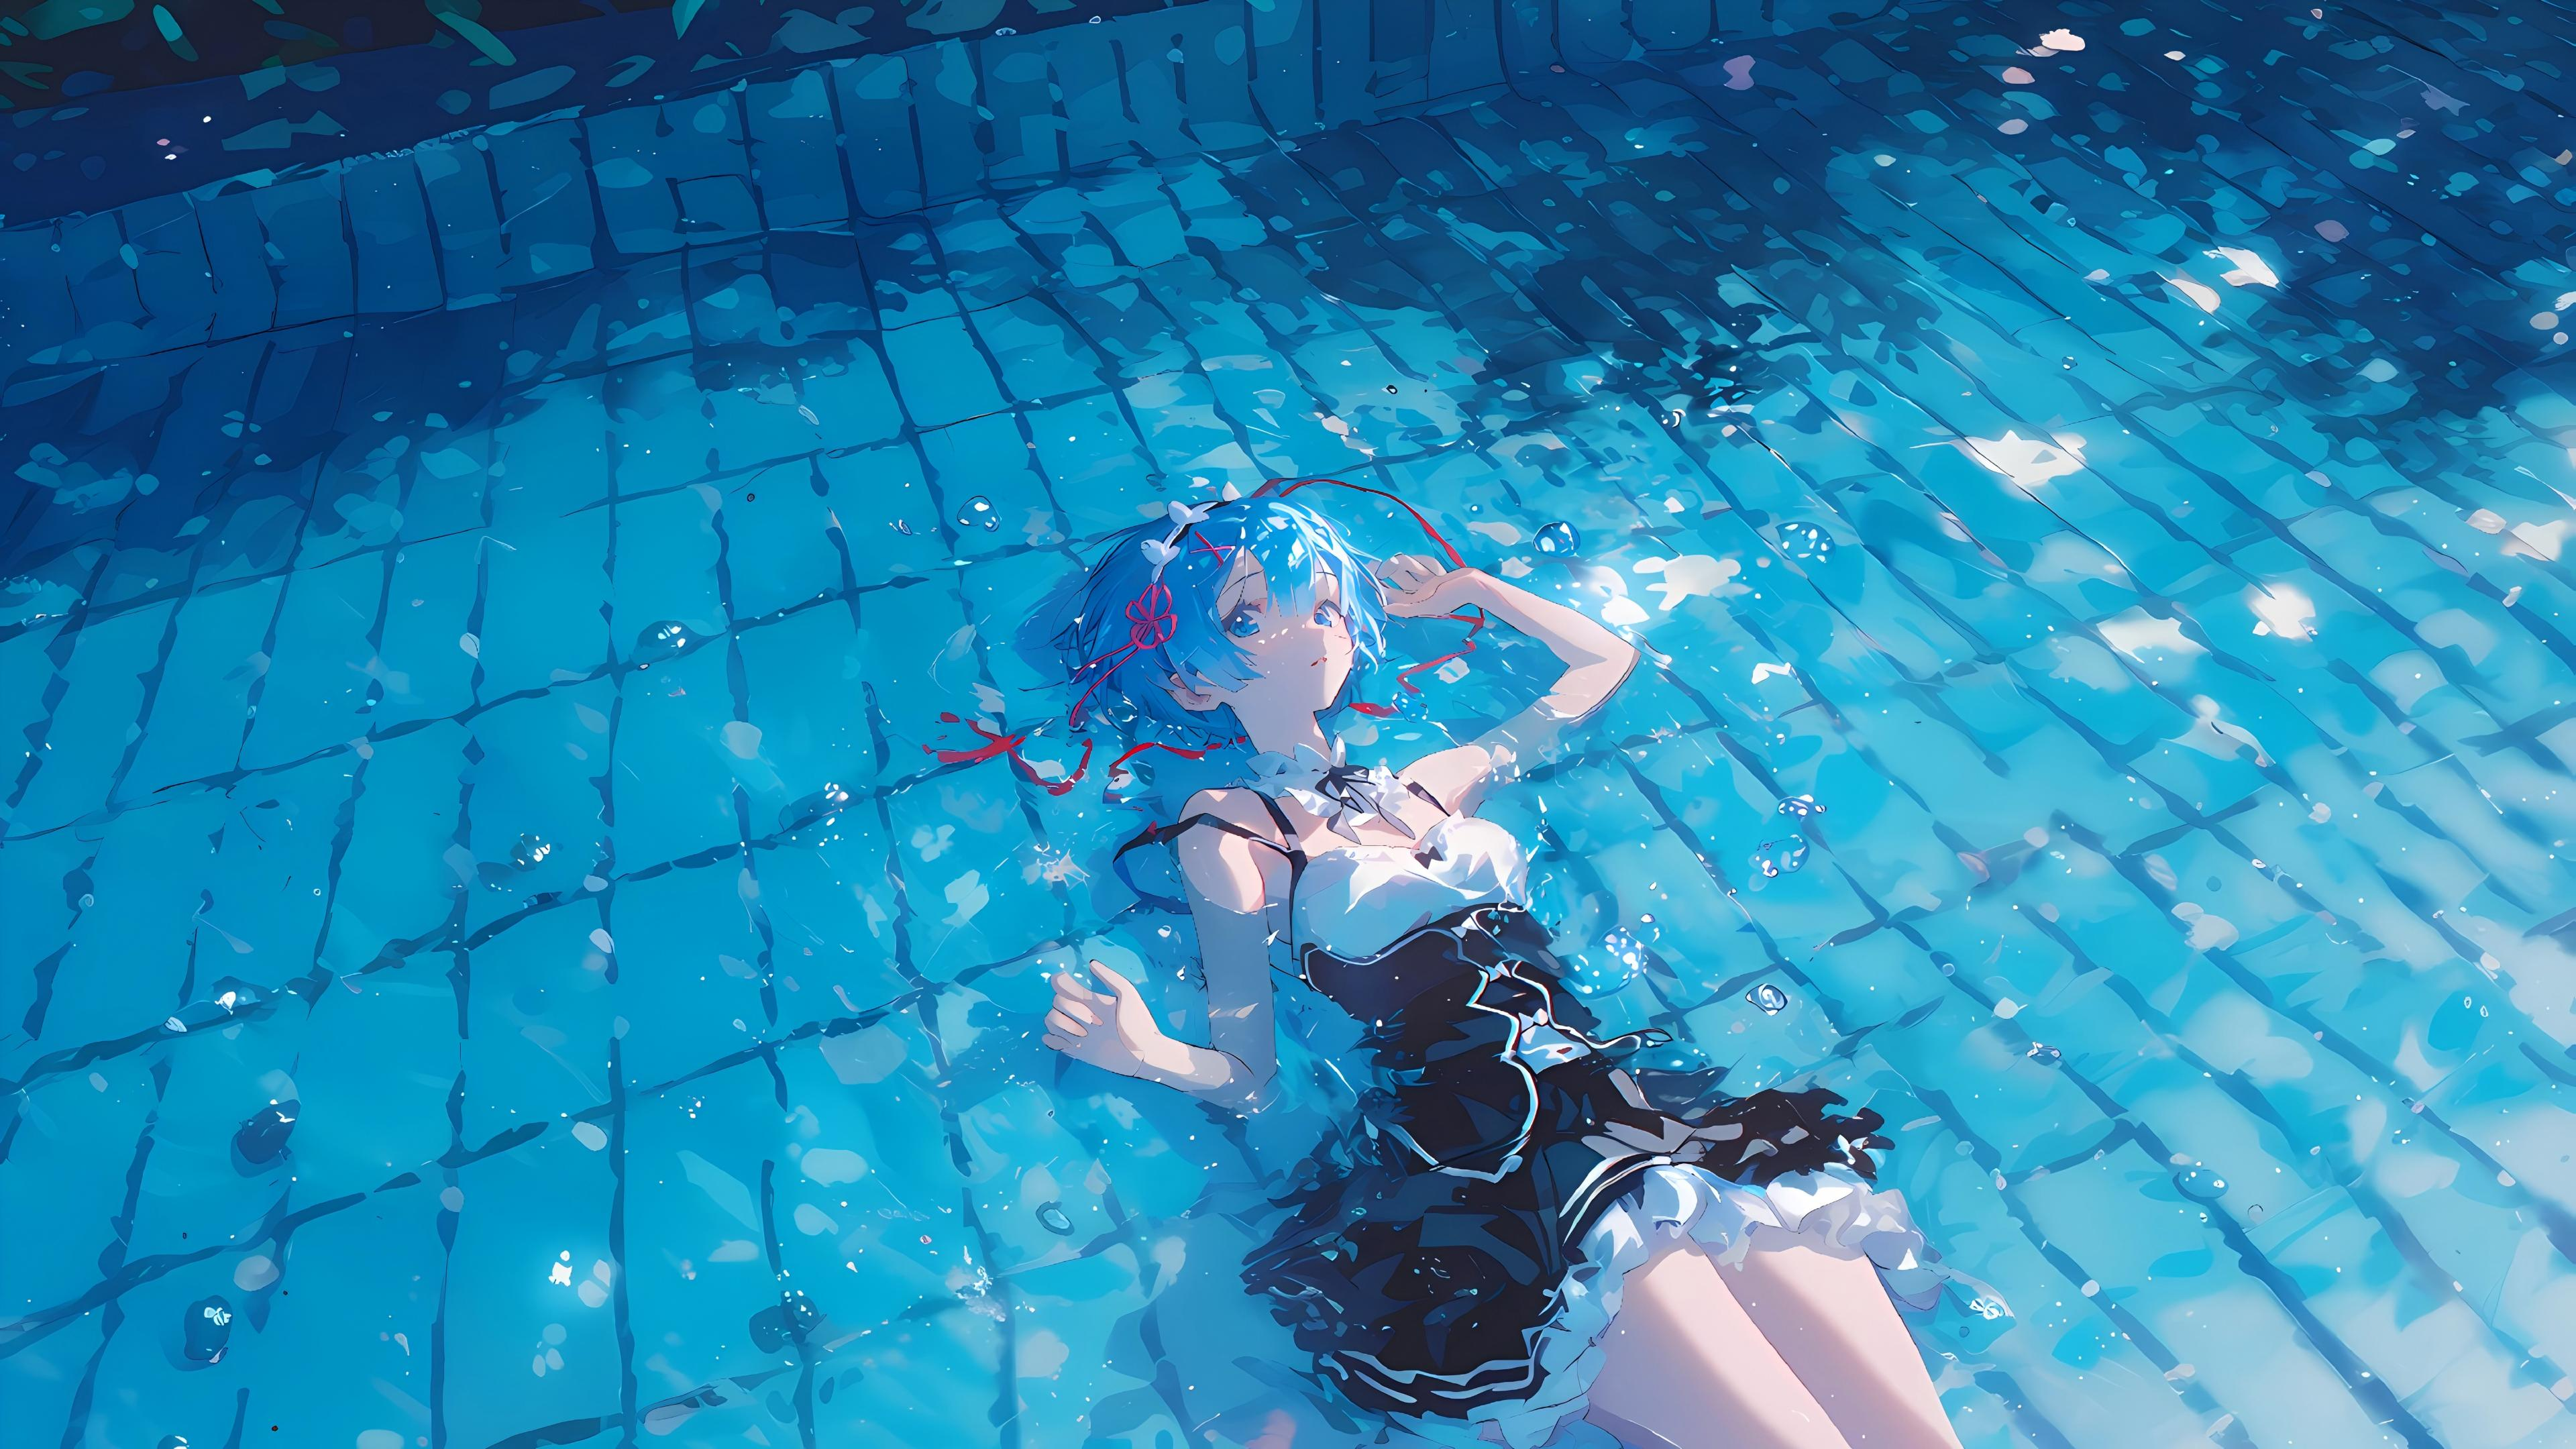
\includegraphics[width=16cm]{figure/封面(1).jpg} % ← 换成你的图片文件
				\end{minipage}
			};
		\end{tikzpicture}
	\end{titlepage}
	% 目录
	\tableofcontents
	
	% 引入章节
	
	\mainmatter % 开始正文部分（通常用于 book 文档类）
	\setcounter{page}{1} % 重置页码计数器为 1
	
	\chapter{引言}
\section{推论，命题与词项}
逻辑是研究推论的,推论由命题组成，命题由词项组成.
\begin{mydefinition}{命题的定义}{}
	 \textbf{命题}是通过语句反映事物情况的思维形式.当你对事物做出肯定或否定的判断时，就构成了命题.例如，“北京是中国的首都”和“雪是黑色的”都是命题.
	
	\textbf{命题的特征}
	\begin{enumerate}
		\item 任何命题要么为真，要么为假
		\item 必须对事物的情况有所断定
	\end{enumerate}
	
	\textbf{直言命题}是直接对对象具有或不具有某种属性做出断定的命题.它不带任何条件，也不需要关系，所以叫“直言”（直接断言）.
	
	\textbf{例子}
	\begin{enumerate}
		\item 所有的金属都是导体.
		\item 有些人不是善良的.
		\item 鲁迅是作家
	\end{enumerate}
\end{mydefinition}

\textbf{直言命题的结构}
任何一个完整的直言命题都由四个部分构成：
\begin{itemize}
	\item 主项：表示被断定的对象（通常用S表示）。如例句中的“金属”、“人”、“鲁迅”。
	\item 谓项：表示被断定具有或不具有的属性（通常用P表示）。如例句中的“导体”、“善良的”、“作家”。
	\item 	联项：表示肯定或否定（即“是”或“不是”）。这是命题的“质”。
	\item 量项：表示主项被断定的数量范围（即“所有”、“有些”、“这个”）。这是命题的“量”。
\end{itemize}
命题是由词项构成的，词项是构成命题的最小意义单位
\begin{mydefinition}{词项的定义}{}
	在逻辑学中，\textbf{词项}指直言命题的主项和谓项，是构成命题的最小意义单元。例如，在“所有金属都是导体”中，“金属”和“导体”就是两个词项。
\end{mydefinition}
词项不等于词或词语，它具有明确的逻辑内涵。同一个词语在不同语境中可能代表不同的词项（如“人”在“人是理性的”和“人是哺乳动物”中侧重点不同）；反之，不同词语也可能表达同一个词项（如“父亲”和“爸爸”）。

词项的\textbf{基本特征}
\begin{itemize}
	\item \textbf{内涵}：词项所反映的事物的特有属性（即“是什么”）。如“人”的内涵是“能制造和使用工具的高等动物”。
	\item \textbf{外延}：词项所指称的一个或多个对象（即“有哪些”）。如“人”的外延包括古今中外的所有人。
\end{itemize}

\textbf{词项的种类}
根据外延的不同，词项通常分为：
\begin{itemize}
	\item \textbf{普遍词项}：外延包含一类以上事物（如“国家”、“书”）。
	
	\item\textbf{单独词项}：外延仅指一个独一无二的事物（如“鲁迅”、“地球”）。
	\item \textbf{空词项}：外延为空，即客观世界不存在对应的事物（如“神仙”、“方的圆”）。
\end{itemize}
\begin{mydefinition}{}{}
	在逻辑学中，\textbf{推论}（Inference）通常是指由已知的一个或几个命题（前提）推导出一个新命题（结论）的思维过程或逻辑形式，是一个能够推出关系的句群
	
\end{mydefinition}
\textbf{推论的基本结构}
\begin{itemize}
	\item \textbf{前提}：作为推理出发点的已知命题。
	\item \textbf{结论}：由前提推导出来的新命题。
	\item \textbf{推导关系}：前提和结论之间的逻辑联系（通常由“所以”、“因此”等词标识）
\end{itemize}
\textbf{推论的分类}
根据推论的思维进程方向，主要分为三类：
\begin{enumerate}
	\item \textbf{演绎推论}:从一般到个别,具有必然性,前提真则结论必真
	\item \textbf{归纳推论}；从个别到一般,具有或然性,前提真只能增加结论的可靠性，但不能保证结论绝对真
	\item \textbf{类比推论}:从个别到个别,具有或然性,根据两个对象的相似性进行类推
\end{enumerate}
我们姑且以演绎推论为主
\section{推论的有效性和可靠性}
考虑以下两个推论
\begin{equation}\label{例子1}
	\begin{aligned}
		&\text{企鹅都是鸟。}\qquad&\text{企鹅都是鸟。}\\
		&\text{猴子都不是企鹅。}\qquad&\text{麻雀都不是企鹅。}\\
		&\text{所以猴子都不是鸟。}\qquad&\text{麻雀都不是鸟。}
	\end{aligned}
\end{equation}

这是两个不同的推论，但他们具有相同的形式
\begin{equation}\label{例子1 的推论形式}
	\begin{aligned}
		&\text{所有S是P。}\\
		&\text{所有Q不是P。}\\
		&\text{所以Q不是P。}
	\end{aligned}
\end{equation}

这样我们给出推论形式的定义
\begin{mydefinition}{}{}
	一类推论所具有的共同结构，称为推论的\textbf{推论形式}。如\ref{例子1}具备的推论形式形式为\ref{例子1 的推论形式},其中$S,P,Q$等可以替换的字母我们称之为\textbf{变项}，定义为没有确定含义的符号或语词，变项可以为词项，命题或个体等等，变项的变化范围定义为\textbf{变域}。每一个变项都有确定的变域。
	
	除了变项以外，\ref{例子1 的推论形式}中还有“所有”“是”“不是”“所以”等词，我们称之为\textbf{常项}，定义为具有确定含义的符号或语词。
\end{mydefinition}
若变项的变域为命题的集合，则称为命题变项；词项的集合，则称之为词项变项；个体的集合，则称之为个体变项。

\begin{mydefinition}{}{}
	当一个\textbf{演绎推论}的所有前提为真时，其结论必然为真，那么具有这样性质的推论，就是\textbf{有效的}
	
\end{mydefinition}
这里，“当一个\textbf{演绎推论}的所有前提为真时”指的是我们假设这个前提是真的，并且在假设前提是真的情况下考虑其结论是否为真，这里我们不在乎这个前提本身是否为真

例子
\begin{equation}
	\begin{aligned}
		&\text{所有的爬行动物是由肺来呼吸的，}\\
		&\text{蛇是爬行动物，}\\
		&\text{所以，蛇是用肺呼吸的。}
	\end{aligned}
\end{equation}
显然这是一个有效的推论














	\part{命题逻辑}
	%\include{chapters/chapter2}
	%\include{chapters/chapter3}
	%\include{chapters/chapter4}
	%\include{chapters/chapter5}
	
	%\include{chapters/chapter6}
	%\include{chapters/chapter7}
	%\include{chapters/chapter8}
	%\include{chapters/chapter9}
	%\include{chapters/chapter10}
	%\include{chapters/chapter11}
	
\end{document}
